% !TEX encoding = UTF-8
%-----------------------------------------------------------------------
% SCPMA submission: HXMT/HE 1B saturation recovery
% Template files in this directory:
%   2026SCGE.cls   (class)
%   scpma.bst      (bib style)
%   picins.sty     (figure support)
% Reference template (do not edit):
%   scpma_template_reference.tex / .pdf
%
% NOTE: 2026SCGE.cls hard-codes hyperref's `dvipdfm' driver, which clashes
% with pdfTeX. The override below forces `pdftex' driver before the cls
% loads hyperref, so we can compile with the standard pdflatex toolchain.
%-----------------------------------------------------------------------
\PassOptionsToPackage{pdftex}{hyperref}
\documentclass[fleqn]{2026SCGE}
\setlength{\mathindent}{0cm}
\usepackage{bm}
\usepackage{algorithm}
\pdfstringdefDisableCommands{\renewcommand*{\bm}[1]{#1}}

\graphicspath{{figures/}}

\thispagestyle{empty}

\begin{document}
\ensubject{Astronomy}

%%%-------------------------------------------------------------
\ArticleType{Article}
\Year{2026}
\Month{}
\Vol{}
\No{}
\DOI{}
\ArtNo{}
\ReceiveDate{}
\AcceptDate{}

\title{Saturation Recovery for Insight-HXMT/HE Bright Burst Observations from Level-1B Raw Data}{Saturation Recovery for Insight-HXMT/HE 1B Data}

% Corresponding author: \author[N]{Name}{{email@xxx.com}}
% Other author:         \author[N]{Name}{}
\author[1]{Hao-Xuan Guo}{{kuohaoxuanus@outlook.com}}
\author[1]{HXMT Collaboration TBD}{}

\AuthorMark{Guo H X}
\AuthorCitation{Guo H X, et al}

\address[1]{Institute of High Energy Physics, Chinese Academy of Sciences, Beijing 100049, China}

%%%-------------------------------------------------------------
\abstract{TBD --- finalized in Task 16 once Phase E numbers are frozen.
Target length 100--200 words. Structure follows the spec at
\texttt{docs/superpowers/specs/2026-05-06-scpma-submission-design.md} \S2.2:
background (HE saturation, 1K limits) / method (1B reconstruction, LIS,
cross-box shape function) / results (260226A residual, 221009A coverage,
multi-layer cross-validation) / implication (open-source release).}

\keywords{Insight-HXMT, gamma-ray bursts, data reconstruction, FIFO saturation, time reconstruction}

\maketitle

%%%=============================================================
\begin{multicols}{2}

\section{Introduction}\label{sec:intro}

The High-Energy detector (HE) on board Insight-HXMT~\cite{zhang2020} provides
$\sim 5100~\mathrm{cm^2}$ of effective area in the 20--250~keV band, which is
among the largest in orbit and makes the instrument uniquely sensitive to
bright hard X-ray and soft $\gamma$-ray transients.\Authorfootnote{} Through its mission HE has
observed many of the brightest events of the past decade, including the
magnetar giant flare GRB~200415A~\cite{roberts2021}, the FRB-associated burst
from SGR~1935$+$2154~\cite{li2021frb}, and the brightest gamma-ray burst ever
recorded, GRB~221009A~\cite{burns2023boat,an2023hxmt}. The same property that
makes HE valuable for these observations---large effective area in a single
collecting volume---also makes it especially prone to electronics-level
saturation. When the photon rate exceeds the readout capacity of the front-end
microcontroller, hardware FIFO buffers overflow, the FPGA side stops accepting
new events, and a fraction of the burst photons are lost without any flag in
the downlinked data.

The standard 1K-level data pipeline accepts this loss as inherent and applies
conservative event-filtering rules in saturated intervals to prevent timing
artifacts from contaminating downstream science. This is appropriate for
routine analysis but discards events that, given the right offline
processing, can in fact be recovered. The lower-level 1B-level raw telemetry
retains the complete CCSDS packet structure, the original 19-bit hardware
time counter (\textit{ptime}), the second-tag events (SEC) used to anchor
absolute time, and every event that passes a 4-bit CRC---including some that
the 1K pipeline subsequently drops at the saturation boundaries.

Reconstructing these events directly from 1B raw data presents two technical
obstacles. First, the ptime counter wraps every $\sim 1.05$~s and the
absolute MET assignment requires knowing how many wrap periods have elapsed
since the most recent SEC anchor. In saturation, FIFO resets and corrupted
SECs make this wrap count locally indeterminate. Second, the 4-bit CRC has a
$1/16$ collision probability, so during long, dense saturation epochs a
substantial fraction of corrupted bytes pass the CRC check and appear as
``ghost events'' with random ptime values---values that, if accepted blindly,
break the strict monotonicity of the underlying FIFO event order and
catastrophically derail naive time-reconstruction algorithms.

We address both obstacles with a single observation: the FIFO is strictly
order-preserving, so the ptime values of \textit{real} events between two
valid SECs must form a strictly increasing sequence under the correct wrap
assignment. The longest increasing subsequence (LIS) of the observed ptime
values therefore identifies the genuine event subset and excludes ghosts
automatically, without thresholding or iterative refinement. Building on
this, we recover events lost to FIFO resets by combining the reconstructed
1B event stream from one detector box with simultaneous unsaturated data
from the other two. The resulting pipeline is validated through three
independent layers---internal 1B/1K consistency checks, comparison against
HE's own engineering-data event counters, and cross-satellite light-curve
matching against Fermi/GBM~\cite{meegan2009gbm},
GECAM-C~\cite{li2022gecam}, and INTEGRAL/SPI-ACS~\cite{savchenko2017spiacs}.

This work makes four contributions:
\begin{itemize}
\item An LIS-based event-level time reconstruction for 1B data that is
intrinsically robust to CRC-collision ghost events, eliminating the cascade
failures observed in greedy alternatives.
\item A grouped-LIS extension with UTC-tail constraints that resolves the
ptime wrap ambiguity introduced by lost SECs, with provable uniqueness for
SEC gaps up to ${\sim}10$~s.
\item A multi-layer validation strategy that exploits HE's three independent
detector boxes and its in-flight engineering counters to bound systematic
errors of the recovery without invoking external instruments.
\item A quantitative characterization of the method's limits, identifying
the failure modes (sub-millisecond burst structure, three-box co-saturation,
and SEC gaps beyond ${\sim}10$~s) and giving the regime within which 1B
recovery can be relied upon for science analyses.
\end{itemize}

The pipeline is implemented in Rust as an open-source command-line tool
released under the MIT license; the corresponding repository is referenced
in the Code and Data Availability statement. Section~\ref{sec:instrument}
describes the HE data system and saturation mechanisms;
Section~\ref{sec:method} details the time-reconstruction algorithm;
Section~\ref{sec:recovery} covers FIFO-reset detection and light-curve
recovery; Section~\ref{sec:validation} presents the three-layer validation;
Section~\ref{sec:discussion} characterizes the method's failure modes; and
Section~\ref{sec:conclusion} summarizes.

\section{HE Data System and Saturation Mechanisms}\label{sec:instrument}

This section describes the HE data acquisition chain at the level of detail
relevant to the 1B reconstruction problem. Readers familiar with the HE
hardware (see~\cite{liu2020he} for a full description) may skim this
section and proceed to Section~\ref{sec:method}. The novel content here is
the explicit characterization of the two saturation loss modes (Section~%
\ref{sec:loss_modes}) and the contrast between 1B raw and 1K processed
data products (Section~\ref{sec:1b_vs_1k}).

\subsection{Hardware data path}\label{sec:datapath}

HE comprises 18 NaI(Tl)/CsI(Na) phoswich detector modules grouped into
three independent boxes (A, B, and C, six modules each) with separate
front-end electronics, FPGAs, microcontrollers, and downlink paths%
~\cite{liu2020he}. Figure~\ref{fig:datapath} traces an event from
detection through downlink. After ASIC digitization, the FPGA writes each
event into a hardware first-in-first-out (FIFO) buffer (FIFO~A, capacity
$\sim 4096$~bytes, holding up to ${\sim}455$ events of 9~bytes each). FIFO~A
is strictly order-preserving, and---critically---when full, additional
writes from the FPGA side are blocked: \textit{the existing buffer
contents are not overwritten and the new events are dropped without any
hardware flag}. An 8051-architecture microcontroller (MCU) reads FIFO~A
in a polling main loop. Each pass invokes \texttt{HandlePhysicalLVDS()},
which extracts up to 109 events, packages them into one CCSDS packet (6-byte
header, $109\times 8 = 872$-byte payload, 4-byte UTC tail; 882 bytes total),
and writes the packet to FIFO~B. Each \texttt{HandlePhysicalLVDS()}
invocation takes $\sim 7$~ms, so the steady-state throughput ceiling is
${\sim}109/7~\mathrm{ms}\approx 15{,}600$ evt/s per box.

\begin{figure}[H]
\centering
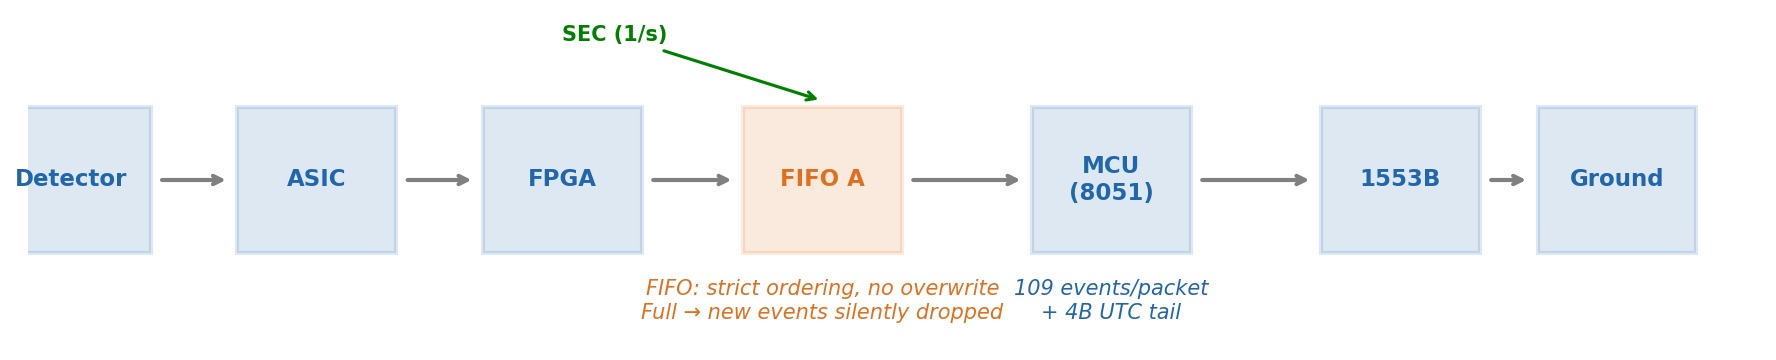
\includegraphics[width=\columnwidth]{f1_datapath.pdf}
\caption{HE data path. Each of the three independent detector boxes
(A, B, C) routes events through ASIC $\to$ FPGA $\to$ FIFO~A
(${\sim}455$~event capacity, strictly FIFO-ordered, no overwrite when full)
$\to$ MCU (8051 polling main loop) $\to$ FIFO~B $\to$ 1553B downlink.
Saturation occurs when the source rate exceeds the MCU's
$\sim 15{,}600$~evt/s readout ceiling, leading to either silent drops at
the FIFO~A write port or full-FIFO resets initiated by the MCU when it
detects sustained overflow.}
\label{fig:datapath}
\end{figure}

\subsection{Event packet format and time stamps}\label{sec:event_format}

Each 8-byte event slot in a CCSDS packet carries:
(i)~event \textit{type} flags identifying physical events (EVT) versus
hardware-injected second markers (SEC) versus error placeholders;
(ii)~for EVT, a 7-bit detector identifier (which together with the box
index determines the 18-detector global ID) and a 7-bit pulse-height
channel; (iii)~for SEC, a 32-bit absolute MET second counter
(\textit{stime}); and (iv)~a 19-bit hardware time counter (\textit{ptime})
plus a 4-bit cyclic-redundancy code (CRC). The ptime counter increments at
$\Delta t = 2~\mu$s per tick and wraps every $P_{\rm MOD} = 2^{19} = 524{,}288$
ticks, i.e., $T_{\rm wrap} \approx 1.0486$~s. SEC events are injected by
the FPGA exactly once per second and provide $(t_{\rm SEC}, p_{\rm SEC})$
anchor pairs for absolute time reconstruction. Both EVT and SEC traverse
the same FIFO~A, so they share its order-preservation and saturation
behavior; in particular, SECs can be lost or corrupted under saturation
just as EVTs can. The 4-byte UTC tail at the end of each packet records
the GPS time at which the MCU \textit{completed} the packet---which can
lag the events themselves by many seconds during deep saturation when
FIFO~A drains slowly.

The 4-bit CRC has a $1/16 \approx 6.3\%$ collision probability, so even
when a transmission error corrupts an event byte, the corrupted value has
a $6.3\%$ chance of passing CRC and being accepted as a valid event with
random ptime and channel. Under nominal conditions this rate is negligible,
but in deep saturation (notably GRB~221009A) the CRC error rate exceeds
$50\%$, generating millions of these ``ghost events'' whose random ptime
values are statistically guaranteed to fall in the gaps of any genuine
event sequence. Section~\ref{sec:method} addresses this directly.

\subsection{Saturation modes: FIFO resets and silent drops}\label{sec:loss_modes}

When the source rate $r$ approaches or exceeds the MCU readout ceiling,
two distinct loss mechanisms appear.

\textbf{(i) FIFO reset (gap loss).} The MCU's main loop includes a
\texttt{FIFOAFullReset()} check: after completing a packet write to FIFO~B,
if FIFO~A is still at maximum fill, the MCU clears the entire FIFO~A
buffer in a single hardware operation, discarding all queued events.
This loses ${\sim}455$ events at once, producing a packet-to-packet gap
in event time that is several times longer than the MCU's normal
$\sim 7$~ms cadence. FIFO resets are detectable from the data because
they leave a gap in MET between consecutive packets that exceeds the
local rate by orders of magnitude---this is the basis of the gap detector
in Section~\ref{sec:detect}.

\textbf{(ii) Silent drop (instantaneous loss).} While the MCU is inside
\texttt{HandlePhysicalLVDS()} for the $\sim 7$~ms required to extract 109
events, FIFO~A briefly fills, the FPGA stops writing, and during this
window any incoming event is dropped. When the MCU finishes the read and
returns to the main loop, FIFO~A is no longer full, so the
\texttt{FIFOAFullReset()} check does not trigger, and the silent drop
leaves no hardware flag. We discuss in Section~\ref{sec:silent_drop} why
silent drops cannot be reliably detected from the data alone, and why their
contribution to total event loss is negligible compared with FIFO resets
in deep saturation.

\subsection{1B versus 1K data products}\label{sec:1b_vs_1k}

The 1B data product is the lowest level of HE telemetry preserved by the
mission archive: it consists of the raw CCSDS packets as downlinked from
the spacecraft, with all CRC information, both EVT and SEC events, and the
UTC tail intact. The 1K product is the standard science-grade output: it
applies time reconstruction, CRC filtering, and conservative event-removal
heuristics around saturation boundaries to yield a clean event list with
absolute MET. The 1K time reconstruction is mature and accurate in
non-saturated intervals, and we do not improve upon it there. What 1K
discards, however, is precisely the population we wish to recover: events
near FIFO-reset boundaries that the heuristics cannot confidently assign,
and events in deep-saturation intervals where SEC anchors are themselves
suspect. This work operates on 1B raw packets, performs an event-level
time reconstruction tailored to the saturation regime, and recovers the
events that 1K conservatively filters out.

\section{Event-Level Time Reconstruction}\label{sec:method}
%% Task 8
TBD --- $\sim$2.5 pages. Opens with framing as prerequisite for
Section~\ref{sec:recovery}.
Subsections 3.1 problem / 3.2 SEC validation / 3.3 $\Delta s_{\rm time}=1$ direct LIS
(includes dead-zone safeguard sentence) / 3.4 $\Delta s_{\rm time}>1$ grouped LIS.

\section{FIFO Reset Detection and Light Curve Recovery}\label{sec:recovery}
%% Task 10 --- HEADLINE SECTION
TBD --- $\sim$2 pages. Opens with ``With per-event times reconstructed, we
address the headline problem''. Subsections 4.1 adaptive gap threshold /
4.2 unreliable interval flagging / 4.3 cross-box shape function /
4.4 three-box co-saturation degenerate case.

\section{Validation}\label{sec:validation}
%% Task 12
TBD --- $\sim$3 pages. Subsections 5.1 internal 1B/1K consistency /
5.2 HE engineering data \textbf{(headline)} / 5.3 cross-satellite (5.3.1
time systems / 5.3.2 GBM / 5.3.3 SPI-ACS / 5.3.4 GECAM-C) /
5.4 cross-box cross-correlation.

\section{Discussion: Limits and Failure Modes}\label{sec:discussion}
%% Task 14
TBD --- $\sim$1.5 pages. Subsections 6.1 too bright / 6.2 too short /
6.3 silent drops (mechanism real but undetectable) / 6.4 CRC-failed event
recovery infeasibility. \textbf{Dead zone is NOT discussed here} ---
it appears only in \S\ref{sec:method} as a boundary safeguard.

\section{Conclusion}\label{sec:conclusion}
%% Task 15
TBD --- $\sim$0.5 pages. Four-bullet summary mirroring contribution list,
plus open-source pointer.

\section*{Code and Data Availability}
%% Task 19
TBD --- statement to be filled with Zenodo DOI after release tag.

%%%=============================================================
%%% References, scpma.bst style
\bibliographystyle{scpma}
\bibliography{refs_en}

\end{multicols}

\end{document}
